\section{Introduction}

\hidenum
\begin{frame}[noframenumbering]
\frametitle{Contents}
 \tableofcontents[currentsection,hideothersubsections,sectionstyle=show/hide]
\end{frame}
\shownum

\subsection{A Concise Introduction to Parallelism}

\begin{frame}
  \begin{block}{What is Parallelism?}\pause
  Broadly, \emph{doing more than one thing at a time}.\\[.2cm]
  
  The simultaneous use of multiple compute resources to solve a computational problem: 
  \end{block}
\end{frame}

\begin{frame}
  \begin{block}{Parallelism}\pause
    \begin{center}
    \begin{minipage}{.46\textwidth}
    \begin{block}{\centering Serial Programming}
      \begin{center}
      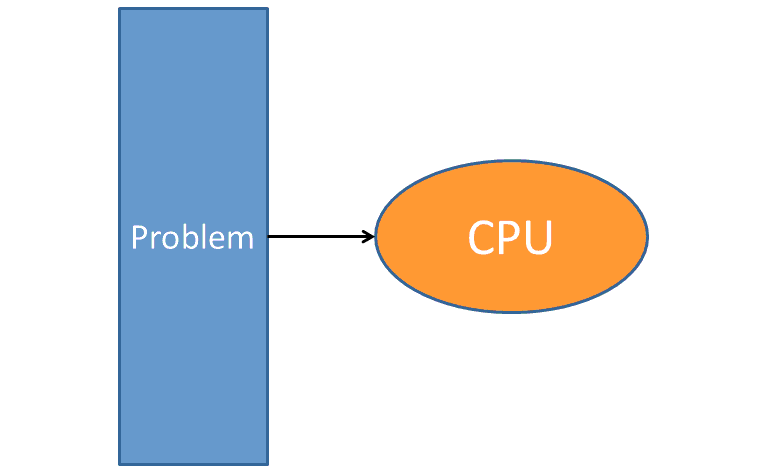
\includegraphics[width=.975\textwidth]{pics/parallelism1}
      \end{center}
      \end{block}
    \end{minipage}
    \hspace{.15cm}
    \begin{minipage}{.46\textwidth}
    \begin{block}{\centering Parallel Programming}
      \begin{center}
      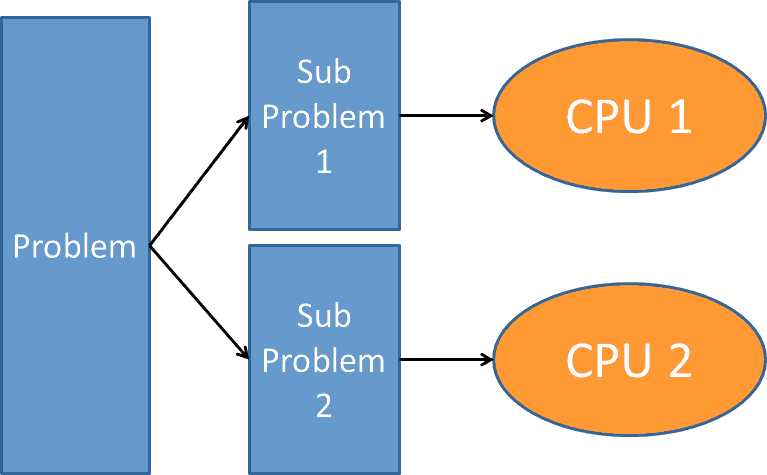
\includegraphics[width=.975\textwidth]{pics/parallelism2}
      \end{center}
      \end{block}
    \end{minipage}
    \end{center}
  \end{block}
\end{frame}

\begin{frame}
  \begin{block}{Parallelism}\pause
    \begin{center}
    \begin{minipage}{.46\textwidth}
    \begin{block}{\centering Serial Programming}
      \begin{center}
      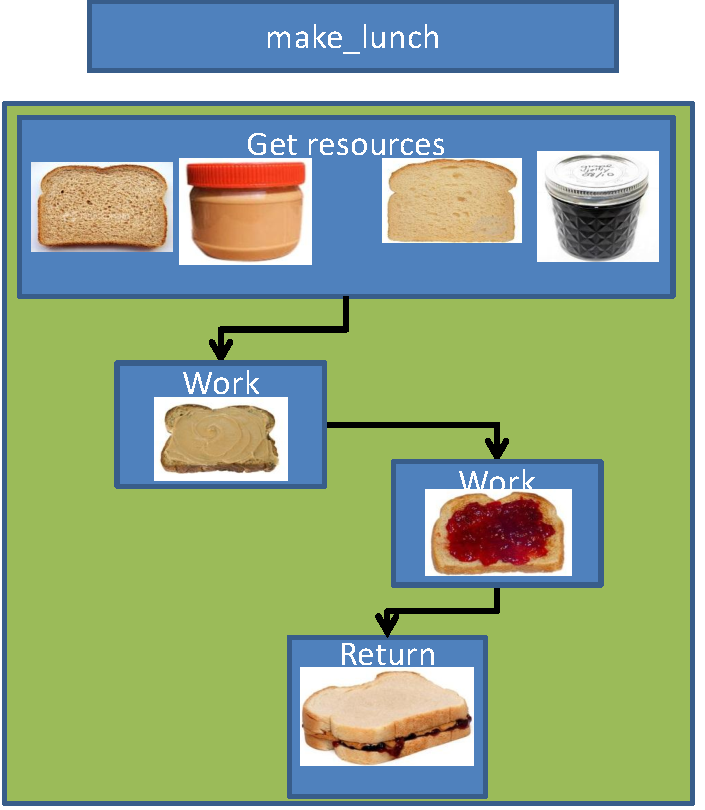
\includegraphics[width=.975\textwidth]{pics/analogy_serial}
      \end{center}
      \end{block}
    \end{minipage}
    \hspace{.15cm}
    \begin{minipage}{.46\textwidth}
    \begin{block}{\centering Parallel Programming}
      \begin{center}
      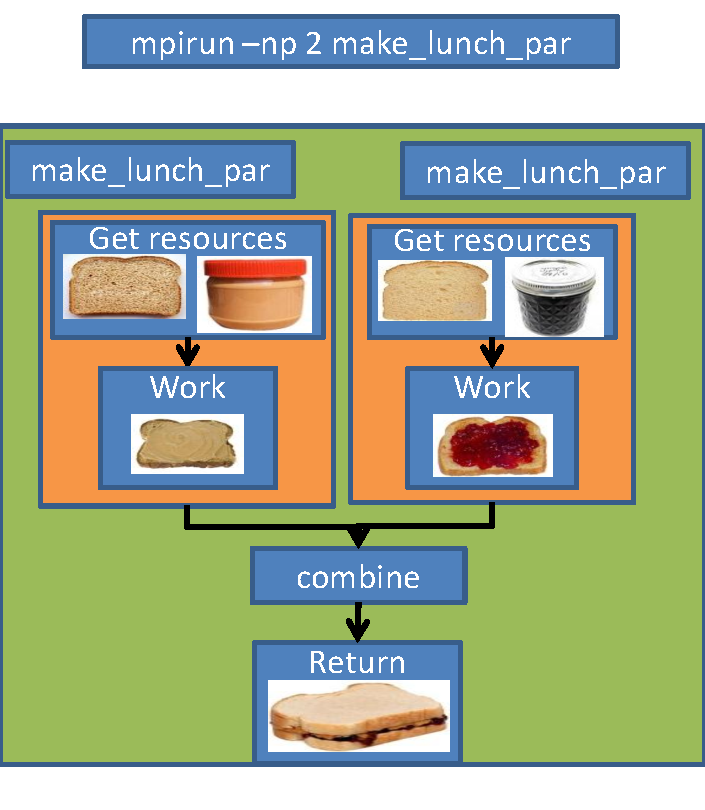
\includegraphics[width=.975\textwidth]{pics/analogy_parallel}
      \end{center}
      \end{block}
    \end{minipage}
    \end{center}
  \end{block}
\end{frame}

% \begin{frame}
%   \begin{block}{What is Parallelism?}\pause
%   Broadly, \emph{doing more than one thing at a time}.\\
%     \begin{itemize}[<+-|alert@+>]
%    \item \emph{Task Parallelism}:  Many small tasks.\\
%    \emph{e.g.} Make one sandwich for each person on earth.
%    \item \emph{Data Parallelism}:  One really big task.\\
%    \emph{e.g.}  Make one sandwich so large that every person on earth could eat from it.\\
%   \end{itemize}
%   \end{block}
% \end{frame}

\begin{frame}
  \begin{block}{What is Parallelism?}\pause
    \begin{itemize}[<+-|alert@+>]
   \item \emph{Task Parallelism}:  Splitting the problem by task
   \item \emph{Data Parallelism}:  
  \end{itemize}
  \end{block}
\end{frame}


\begin{frame}
  \begin{block}{Data vs Task Parallelism}\pause
    \begin{center}
    \begin{minipage}{.46\textwidth}
    \begin{block}{\centering Data Parallelism}
      \begin{center}
      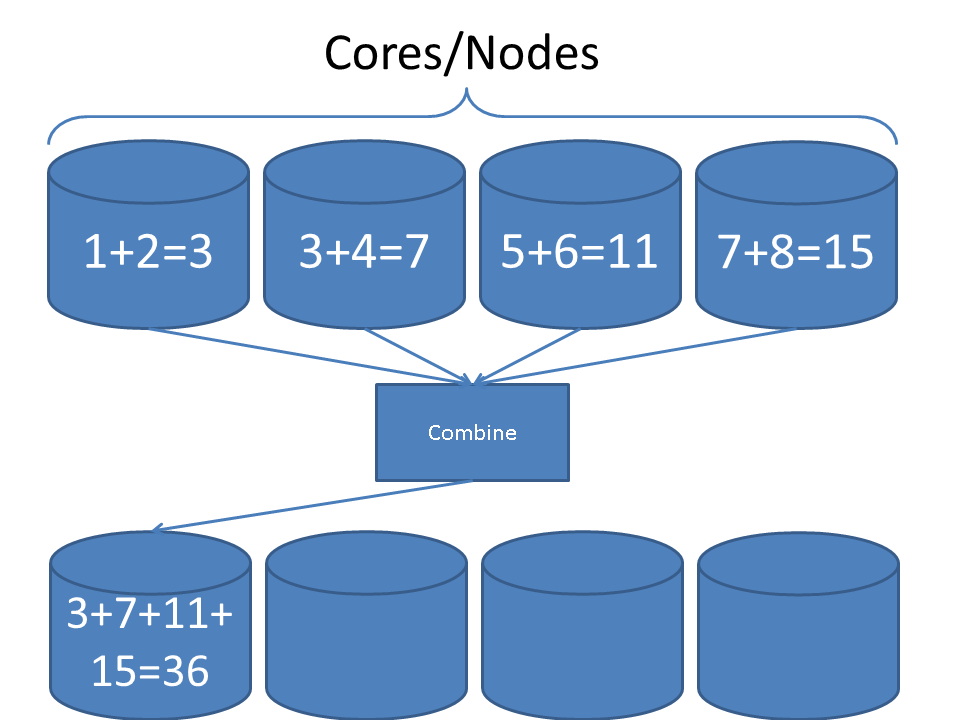
\includegraphics[width=.975\textwidth]{pics/parallelism_data}
      \end{center}
      \end{block}
    \end{minipage}
    \hspace{.15cm}
    \begin{minipage}{.46\textwidth}
    \begin{block}{\centering Task Parallelism}
      \begin{center}
      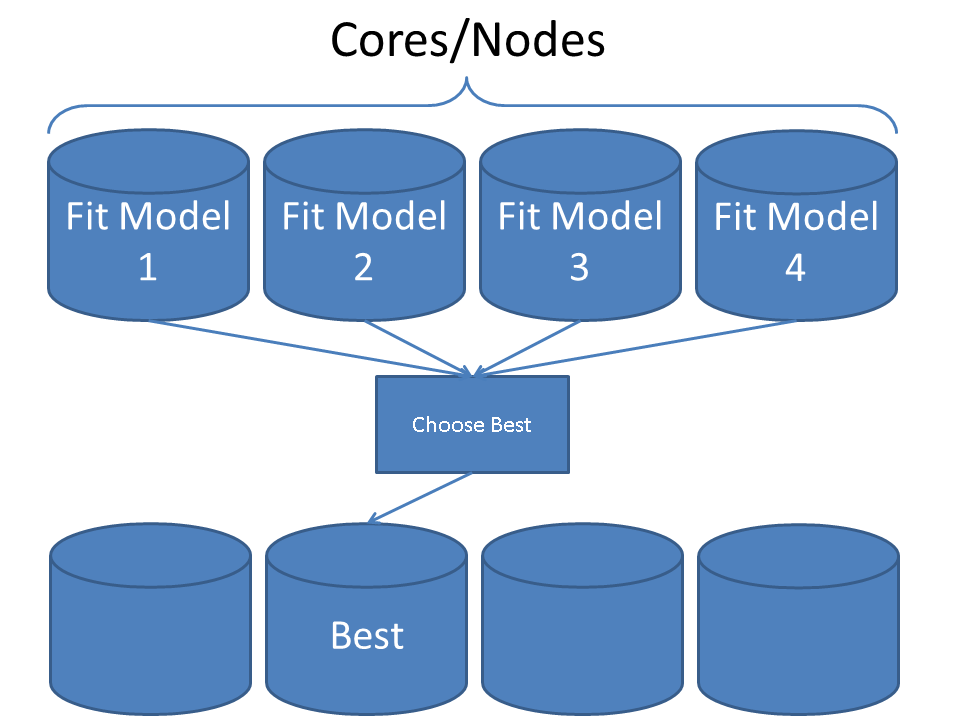
\includegraphics[width=.975\textwidth]{pics/parallelism_task}
      \end{center}
      \end{block}
    \end{minipage}
    \end{center}
  \end{block}
\end{frame}


\begin{frame}
  \begin{block}{Common Terms}
  \begin{enumerate}[<+-|alert@+>]
    \item \emph{Embarrassingly Parallel}:  Also called \emph{loosely coupled}.  Obvious how to make parallel; lots of independence in computations.
    \item \emph{Tightly Coupled}:  Opposite of embarrassingly parallel; lots of dependence in computations.
    \item \emph{Implicit parallelism}:  Parallel details hidden from user
    \item \emph{Explicit parallelism}:  Some assembly required\dots
  \end{enumerate}  
  \end{block}
\end{frame}


\subsection{R and Parallelism}

\begin{frame}[shrink]
  \begin{block}{R and Parallelism}
    The solution to many of R's problems is parallelism.  However \dots\vspace{-.4cm}
   \begin{center}
    \begin{minipage}[t]{.95\textwidth}
    \begin{block}{\centering What we have}
      \begin{enumerate}[<+-|alert@+>]
        \item Mostly serial.
        \item Parallelism mostly not distributed (foreach, parallel/snow/multicore, \dots)
        \item Data parallelism mostly explicit (Rmpi, R+Hadoop, \dots)
      \end{enumerate}
    \end{block}
    \end{minipage}
    \\\pause
    \begin{minipage}[t]{.95\textwidth}
    \begin{block}{\centering What we want}
      \begin{enumerate}[<+-|alert@+>]
        \item Mostly parallel.
        \item Mostly distributed.
        \item Mostly implicit.
      \end{enumerate}
    \end{block}
    \end{minipage}
    \end{center}
    \end{block}
\end{frame}


\begin{frame}
  \begin{block}{Why We Need Parallelism}\pause
    \begin{enumerate}[<+-|alert@+>]
      \item Saves time (long term).
      \item Data size is skyrocketing.
      \item Necessary for many problems.
      \item Like it or not, it's coming.
      \item \emph{It's really cool.}
  \end{enumerate}
  \end{block}
\end{frame}




\begin{frame}
%  \addtocounter{framenumber}{-1}
  \begin{block}{Problems with R}\pause
  \begin{enumerate}[<+-|alert@+>]
    \item Slow.
    \item If you don't know what you're doing, it's \emph{really} slow.
    \item Performance improvements usually for small machines.
    \item Very ram intensive.
    \item Chokes on big data.
  \end{enumerate}
  \end{block}
\end{frame}

